\section{Comparison}
\label{sec:comparison}

First, in Fig.~\ref{fig:timeline1} we provide a timeline which depicts when the particular data generator was introduced.

\begin{figure}[h]
\centering
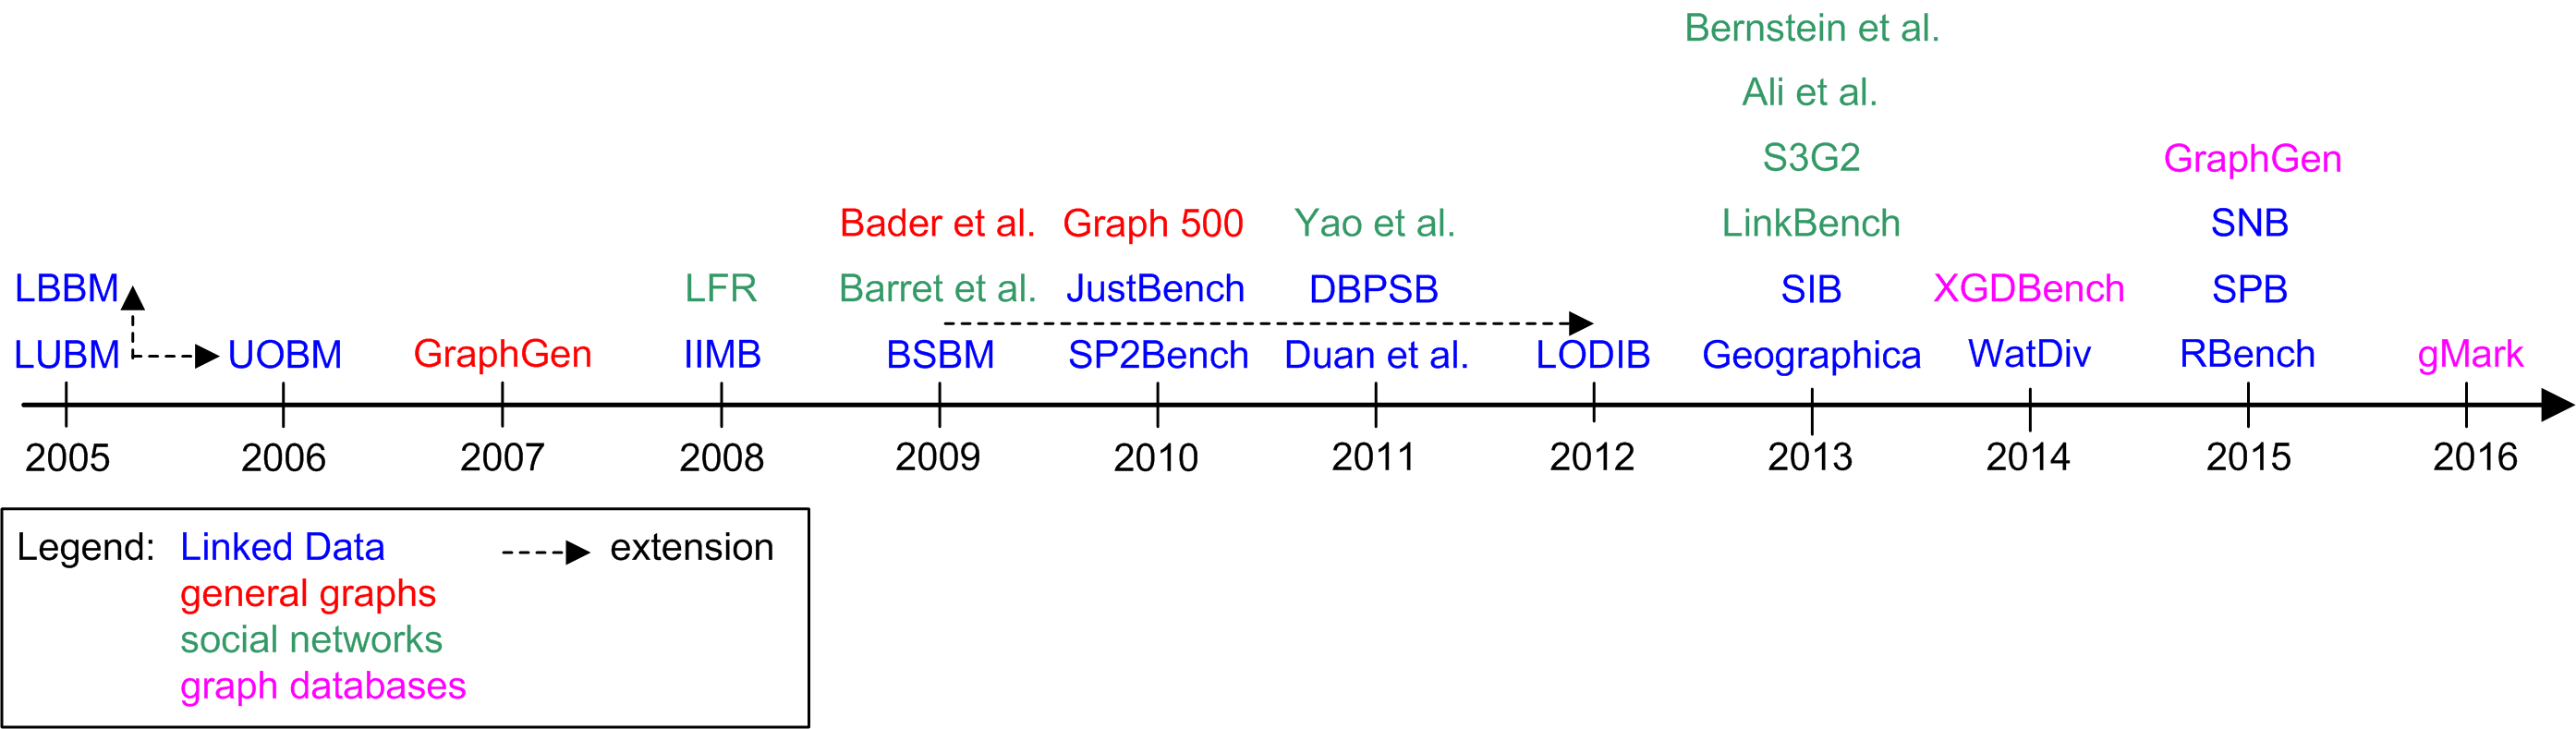
\includegraphics[width=\textwidth]{timeline1.png}
\caption{Timeline}
\label{fig:timeline1}
\end{figure}


Next, in Tables~\ref{tab:comparison_gen_text} to~\ref{tab:comparison_sn_yesno} we compare the functionalities of the generators. We focus on ....

%%%%%%%%%%%%%%%%%%%%%%%%%%%%%%%%%%%%%%%%%%%%%%%

\begin{table}[h]
\footnotesize
\centering
\tbl{Comparison of graph data generators -- general graphs}{
\begin{tabular}{| p{1.9cm} | p{1.2cm} | p{1.5cm} | p{1.3cm} | p{1.5cm} | p{1.5cm} |p{1.5cm} |}
 \hline
               & Graph
               & Parameters
               & Algorithm
               & Output format
               & Operations
               & Problem domain
               \\ \hline \hline
%   &  & & & &   &         \\ \hline
 GraphGen~\cite{GraphGen}   & labelled, undirected, connected & number of graphs, average size of graphs, average density, ... & \NO & list of graphs, their nodes and edges & frequent subgraph mining, query processing  &  \NO       \\ \hline
 HPC Scalable Graph Analysis Benchmark \cite{HPCgraph}  & weighted, directed & number of vertices, number of edges, and maximum weight of an edge & R-MAT & tuples $\langle$ start vertex, end vertex, weight $\rangle$ & classification of large vertex sets, graph extraction with BFS, and graph analysis with betweenness centrality & \NO         \\ \hline
 Graph 500 Benchmark \cite{Graph500} & weighted, undirected & scale, edge factor & R-MAT & tuples $\langle$ start vertex, end vertex, weight $\rangle$ & BFS  & \NO        \\ \hline
\end{tabular} }
\label{tab:comparison_gen_text}
\end{table}

\begin{table}[h]
\footnotesize
\centering
\tbl{Comparison of graph data generators -- Linked Data}{
\begin{tabular}{| p{1.9cm} | p{1.2cm} | p{3cm} | p{1.3cm} | p{3cm} | p{1.5cm} |}
 \hline
               & Graph
               & Parameters
               & Output format
               & Queries
               & Problem domain
               \\ \hline \hline
 LUBM \cite{Guo2005158} & RDF & seed for random number generation, number of universities, starting index of universities & RDF &  14 & storing, querying \\ \hline
 LBBM \cite{Wang2005} & RDF &  number of triples & RDF &  12 & storing, querying \\ \hline
 UOBM \cite{Ma:2006:TCO:2094613.2094629} & RDF & number of universities, probability of generating of various additional links & RDF & 15 & storing, querying  \\ \hline
 IIMB \cite{Ferrara08OM} & RDF & required transformations & RDF & \NO & instance matching \\ \hline
 BSBM \cite{Bizer09theberlin} & RDF & number of products & RDF, relational  & 12 & storing, querying          \\ \hline
 SP$^2$Bench \cite{Schmidt2010} & RDF & triple count / year up to which data is
generated & RDF & 12  &  storing, querying        \\ \hline
 \cite{Duan:2011:AOC:1989323.1989340} & RDF & size, coherence & RDF & \NO    &  storing, querying     \\ \hline
 DBPSB \cite{Morsey2011}     & RDF    & scale factor     & RDF    & 25 derived templates  & storing, querying\\ \hline
 LODIB \cite{DBLP:conf/www/RiveroSBR12} & RDF & number of product instances & RDF & \NO           & translation systems \\ \hline
 SIB \cite{sib} & RDF & number of users & RDF &  3 query mixes    & storing, querying \\ \hline
 Geographica \cite{DBLP:conf/semweb/GarbisKK13} & RDF & size & RDF & 29 + 11 queries + 2 query templates  & geospatial RDF stores    \\ \hline
 WatDiv \cite{Aluc:2014:DST:2717213.2717229}     &  RDF   &  WatDiv schema, scale factor, value distributions, number of query templates, their restrictions  &  RDF   &  user-specified number of query templates and respective query instances & storing, querying \\ \hline
 RBench \cite{Qiao:2015:RAR:2723372.2746479}     &   RDF  &  size + degree scaling factor   & RDF    & 5 types of queries generated for the synthetic data  & storing, querying  \\ \hline
 LDBC SPB \cite{spb}     & RDF   & size     & RDF   & 2 query mixes   & storing, querying \\ \hline
\end{tabular} }
\label{tab:comparison_ld_text}
\end{table}

\begin{table}[h]
\footnotesize
\centering
\tbl{Comparison of graph data generators -- graph databases}{
\begin{tabular}{| p{1.9cm} | p{1.2cm} | p{3cm} | p{1.3cm} | p{3cm} | p{1.5cm} |}
 \hline
               & Graph
               & Parameters
               & Output format
               & Queries
               & Problem domain
               \\ \hline \hline
gMark~\cite{gMark}   & any & graph and query workload configuration & various (e.g., N-triples + SQL, SPARQL, Datalog, openCypher) & synthetically generated  & querying, graph analytics, schema validation         \\ \hline
XGDBench~\cite{Dayarathna:2014:GDB:2676904.2676939}  & any & number of vertices and attributes per vertex, a threshold for random initialization of attributes, an edge affinity threshold, an affinity matrix & DistArray of X10 & 7 workloads & storing, graph operations \\ \hline
\end{tabular} }
\label{tab:comparison_gdb_text}
\end{table}

\begin{table}[h]
\footnotesize
\centering
\tbl{Comparison of graph data generators -- social networks}{
\begin{tabular}{| p{1.9cm} | p{1.2cm} | p{3cm} | p{1.3cm} | p{3cm} | p{1.5cm} |}
 \hline
               & Graph
               & Parameters
               & Output format
               & Queries
               & Problem domain
               \\ \hline \hline
 LFR~\cite{PhysRevE.78.046110}      & social network    & number of nodes, power-law exponents, mixing parameter  & n/a   & \NO    &  community detection    \\ \hline
 \cite{Barrett:2009:GAL:1995456.1995598} & social network & data sets, activity templates & n/a & \NO & analysis        \\ \hline
 \cite{Yao2011}   & linkage graph & burning probability, symmetry probability & n/a & \NO  & degree correlation analysis         \\ \hline
 LinkBench \cite{Armstrong:2013:LDB:2463676.2465296} & social network & number of nodes & MySQL compliant &  10 graph operations  & storing, data access       \\ \hline
 S3G2 \cite{Pham2013} & social network (RDF) & data schema, dictionaries, property value correlations, correlation dimensions  & RDF & \NO & storing, analysis         \\ \hline
 \cite{Sukthankar-SocialInfo2014} & social network & network to be cloned, homophily, link density & n/a & \NO & benchmarking, debugging, simulation   \\ \hline
 LDBC SNB \cite{Erling:2015:LSN:2723372.2742786}     &  social network (RDF)   &  the amount of persons    &  RDF (CSV, Ntriple)   & 3 workloads  &  storing, querying \\ \hline
\end{tabular} }
\label{tab:comparison_sn_text}
\end{table}

%%%%%%%%%%%%%%%%%%%%%%%%%%%%%%%%%%%%%%%%%%%%%%%%%%%%%%%%%%%%%%

\begin{table}[h]
\footnotesize
\centering
\tbl{Comparison of graph data generators -- general graphs (yes/no features)}{
\begin{tabular}{| l | l | l | l | l | l | l | l | }
 \hline
               & \rot{Domain-specific}
               & \rot{Language-specific}
               & \rot{Use-case driven}
               &  \rot{Considering true Big Data}
               \\ \hline \hline
% &  &  &  &            \\ \hline
 GraphGen \cite{GraphGen}  & \NO & \NO & \NO & \OK           \\ \hline
 HPC Scalable Graph Analysis Benchmark\cite{HPCgraph}  & \NO & \NO & \NO & \OK           \\ \hline
 Graph 500 Benchmark \cite{Graph500}     & \NO    &  \NO    & \NO    & \OK    \\ \hline
\end{tabular} }
\label{tab:comparison_gen_yesno}
\end{table}

\begin{table}[h]
\footnotesize
\centering
\tbl{Comparison of graph data generators -- Linked Data (yes/no features)}{
\begin{tabular}{| l | l | l | l | l | l | l | l | }
 \hline
               & \rot{Domain-specific}
               & \rot{Language-specific}
               & \rot{Use-case driven}
               &  \rot{Considering true Big Data}
               \\ \hline \hline
 LUBM \cite{Guo2005158}     & \OK    &  \NO    &  \OK   & \NO     \\ \hline
 LBBM \cite{Wang2005}     & \NO    &  \NO    &   \NO  &  \NO    \\ \hline
 UOBM \cite{Ma:2006:TCO:2094613.2094629}     &  \OK    &  \NO    &  \OK    & \NO     \\ \hline
 IIMB \cite{Ferrara08OM} & \OK & \NO & \OK &  \NO          \\ \hline
 BSBM \cite{Bizer09theberlin}     &  \OK   &  \NO    & \OK    &  \NO    \\ \hline
 SP$^2$Bench \cite{Schmidt2010}     & \OK    &  \OK    & \NO    &  \NO    \\ \hline
 \cite{Duan:2011:AOC:1989323.1989340}     & \NO & \NO  &  \NO   &  \NO    \\ \hline
 DBPSB \cite{Morsey2011}     & \OK    &  \NO    &  \OK   &  \NO    \\ \hline
 LODIB \cite{DBLP:conf/www/RiveroSBR12} & \OK & \NO & \OK &   \NO         \\ \hline
 SIB \cite{sib} & \OK & \OK & \OK &  \NO          \\ \hline
 Geographica \cite{DBLP:conf/semweb/GarbisKK13} & \OK & \OK & \OK & \NO           \\ \hline
 WatDiv \cite{Aluc:2014:DST:2717213.2717229}     &  \OK   & \OK     &  \NO   &   \NO   \\ \hline
 RBench \cite{Qiao:2015:RAR:2723372.2746479}     &  \NO   & \NO     & \NO    & \NO     \\ \hline
 LDBC SPB \cite{spb}     & \OK    & \NO     & \OK    &  \NO    \\ \hline
\end{tabular} }
\label{tab:comparison_ld_yesno}
\end{table}

\begin{table}[h]
\footnotesize
\centering
\tbl{Comparison of graph data generators -- graph databases (yes/no features)}{
\begin{tabular}{| l | l | l | l | l | l | l | l | }
 \hline
               & \rot{Domain-specific}
               & \rot{Language-specific}
               & \rot{Use-case driven}
               &  \rot{Considering true Big Data}
               \\ \hline \hline
Graph 500 Benchmark~\cite{Graph500}     & \NO    &  \NO    & \NO    & \NO     \\ \hline
XGDBench~\cite{Dayarathna:2014:GDB:2676904.2676939}      & \NO    & \NO     &  \NO   & \OK     \\ \hline
%      &     &      &     &      \\ \hline
\end{tabular} }
\label{tab:comparison_gdb_yesno}
\end{table}

\begin{table}[h]
\footnotesize
\centering
\tbl{Comparison of graph data generators -- social networks (yes/no features)}{
\begin{tabular}{| l | l | l | l | l | l | l | l | }
 \hline
               & \rot{Domain-specific}
               & \rot{Language-specific}
               & \rot{Use-case driven}
               & \rot{Considering true Big Data}
               & \rot{Statistical/Agent-based}
               \\ \hline \hline
LFR~\cite{PhysRevE.78.046110}      & \NO    &  \NO    & \NO    & \NO  & S   \\ \hline
 \cite{Barrett:2009:GAL:1995456.1995598} & \NO    &  \NO    & \NO    & \NO  & A   \\ \hline
 \cite{Yao2011}   & \NO  & \NO & \NO  & \NO  & S        \\ \hline
 LinkBench \cite{Armstrong:2013:LDB:2463676.2465296} & \OK & \NO & \OK & \OK & S          \\ \hline
  S3G2 \cite{Pham2013} & \NO & \NO & \NO & \OK & S       \\ \hline
%  \cite{Bernstein:2013:SAS:2499604.2499609} & \NO & \NO & \NO & \OK & A       \\ \hline
 \cite{Sukthankar-SocialInfo2014} & \NO    &  \NO    & \NO    & \NO & S    \\ \hline
 LDBC-SNB \cite{Erling:2015:LSN:2723372.2742786}     &   \OK    & \NO     & \OK    & \OK  & S  \\ \hline
%      &     &      &     &      \\ \hline

\end{tabular} }
\label{tab:comparison_sn_yesno}
\end{table}


As we can see ...
